\ifx \allfiles \undefined
\documentclass{article}
\usepackage{booktabs}
\usepackage{multirow}
\usepackage{graphicx}
\usepackage{subfigure}

\begin{document}
\title{Method}
\maketitle \else \fi

\section{Experiments}\label{sec:experiment}
In this section, we test our different models on real dataset extracted from twitter. We name snowball algorithm as SA, bidirectional snowball algorithm as BSA, naive Bayes algorithm as NBA and the co-training framework that combines bidirectional snowball algorithm and naive Bayes algorithm as CA. In the experiments, we use precision at the position $K$ to evaluate the accuracy of our ranking result. The precision at the position $K$ measures how many related user we ranked in top $K$ positions. The precision at $K$ method penalizes the model which performs poorly in ranking result. Here we didn't use recall as one of our metrics since that we can hardly obtain the exactly number of users belong to our target category.

\subsection{Data Collection}
\textbf{User data:} Twenty seed users were selected from each of the four universities, including UCLA, USC, Stanford and MIT. User profile (id, location, screen name, number of followings and followers, and a short biography) of these seed users was crawled using the Twitter API. Starting from these seed users, a two-step random walk was performed to retrieve their followers and their followers' followers. If a new user from these four universities was discovered during the procedure (the user's short biography contains the university name), this user was marked as a seed user and another two-step random walk starting from this user was performed. The data was collected during October, 2011. The crawler had collected more than $540,000$ users and $780,000,000$ following relations. It had also collected the most recent $40$ tweets for each user, summing up to $15,321,508$ tweets in total. These tweets contains $3,143,115$ different words. Since user word pairs are very sparse and some word appeared in only a few users are not generalizable, we eliminate the words appeared less than $100$ times and there is about $20,000$ word left.

\textbf{Label data:} During our experiments, we mainly focus on ranking users from four categories, they are UCLA, Stanford, MIT and USC. The user belong to these four universities may highly connected with each other. Later in our experiments part, we will prove that some of our algorithm will still have good performance with dataset that is not highly connected. For category of each university, we use $80\%$ users with target keyword in their short bio as training data and erase the target keyword appeared in other $20\%$ users.

\textbf{Human label data:} In the evaluation process, we will also label top $100$ results of different approaches from UCLA category by human in order to obtain a more accuracy evaluation result. During the labeling process, we take into consideration not only users' profile information, but also users' tweets, users' following relationship and search users' names in Google. Besides, as we present a ranking result, we will consider whether a user never log on twitter after he register his account and we may separate user who is belong to this category and who is interest in this category. More detail information about labeling result will discuss in the discussion section.

\subsection{Ranking Performance}
In this part of the experiments, we use our label data and sort the users with respect to the estimated relevance given by our algorithm. We show the detailed precision curve (at different position) on label data for different categories in Figure \ref{fig:e1}.

\begin{figure*}[htb!]
\centering
\subfigure[UCLA]{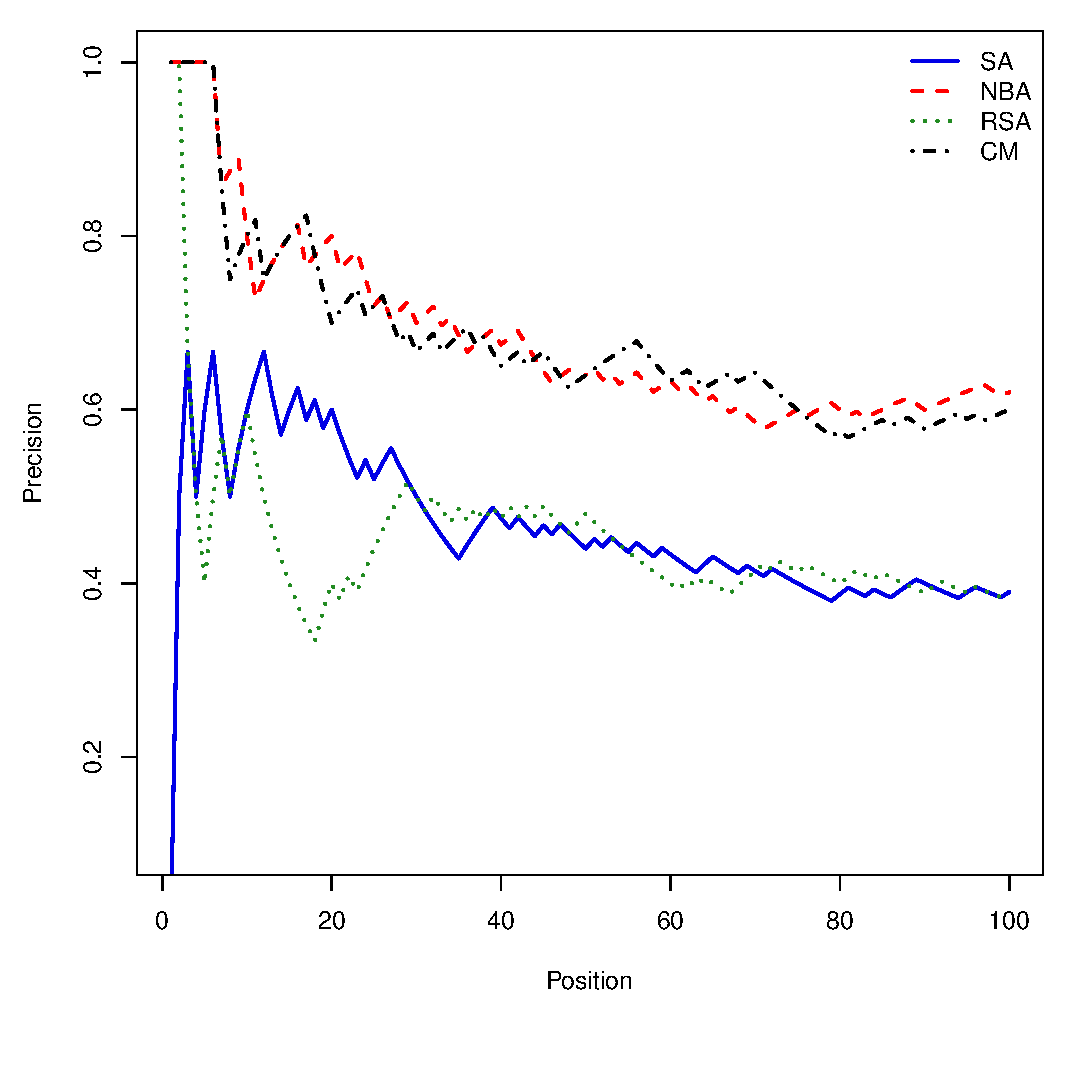
\includegraphics[width=0.45\textwidth]{experiment/e1.ucla.eps}}
\subfigure[MIT]{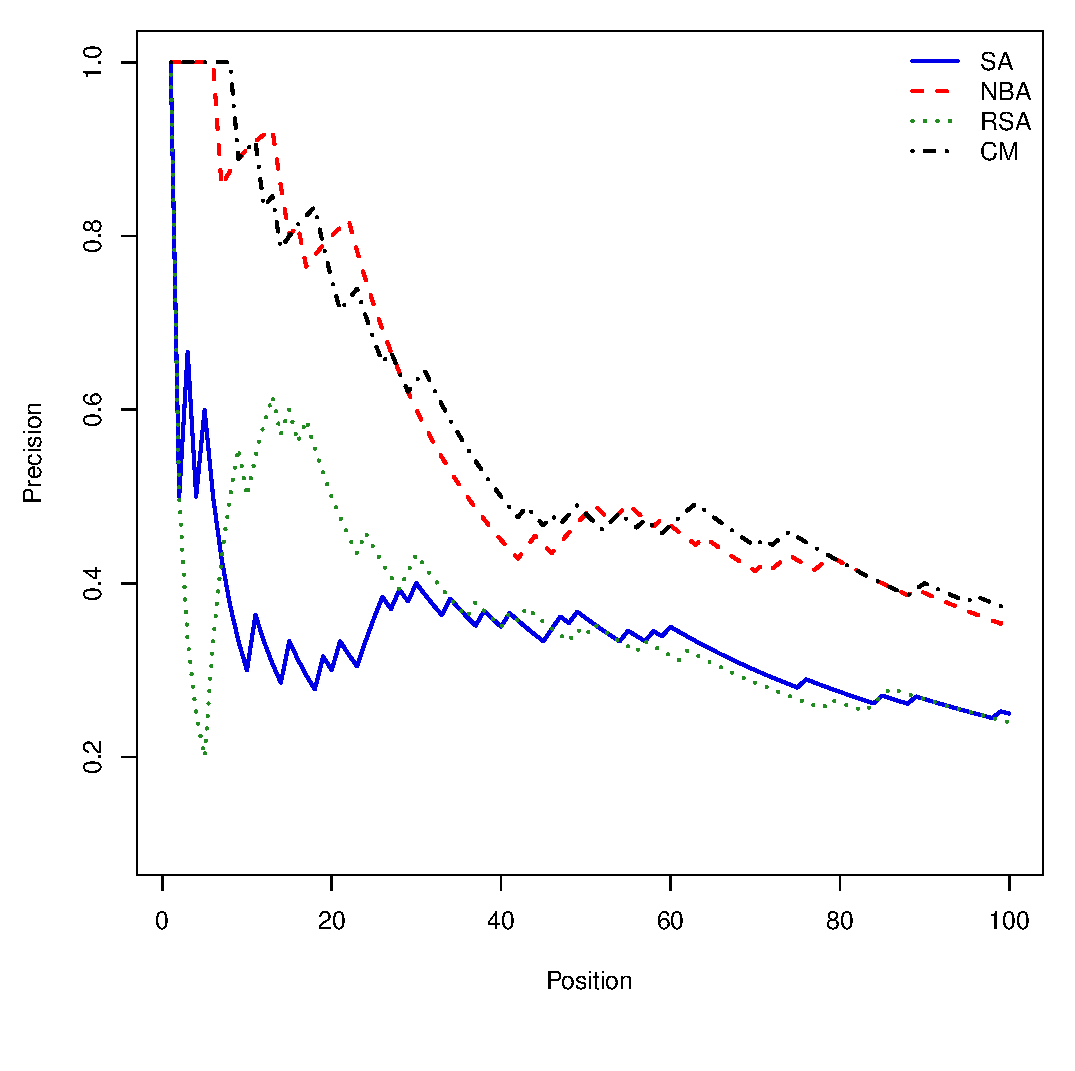
\includegraphics[width=0.45\textwidth]{experiment/e1.mit.eps}}
\\
\subfigure[Stanford]{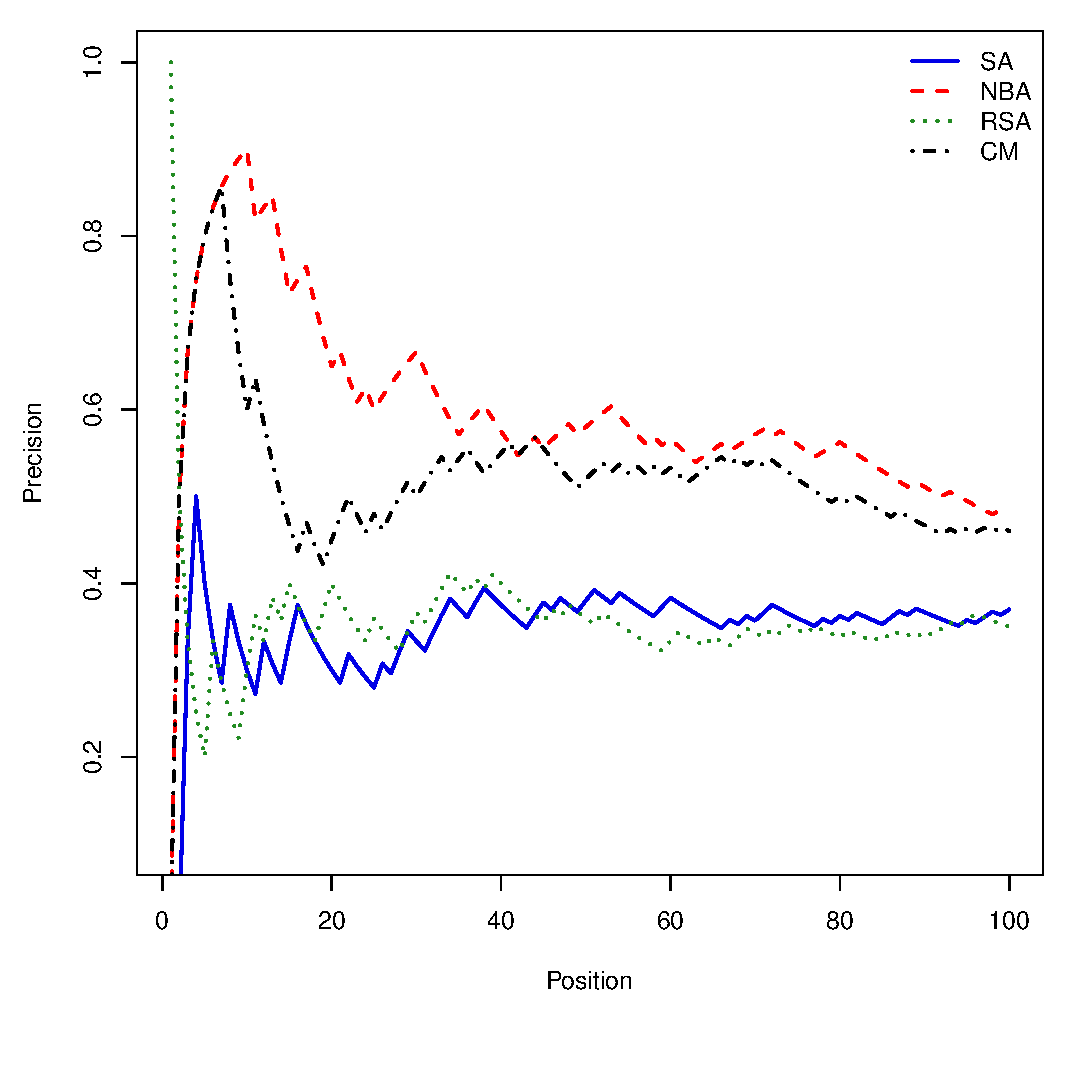
\includegraphics[width=0.45\textwidth]{experiment/e1.stanford.eps}}
\subfigure[USC]{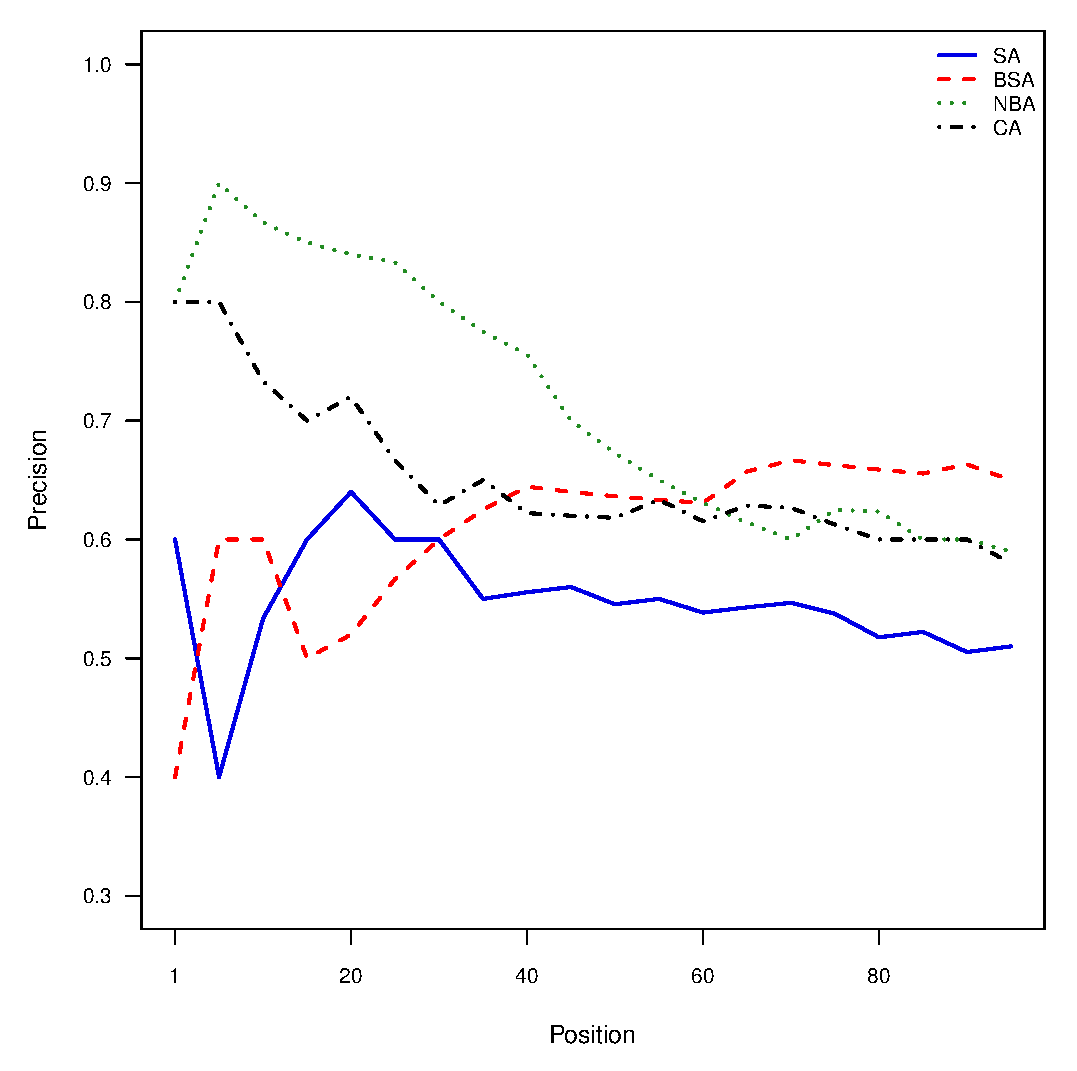
\includegraphics[width=0.45\textwidth]{experiment/e1.usc.eps}}
\caption{Precision@K for different category.}
\label{fig:e1}
\end{figure*}

From Figure \ref{fig:e1} we can see that the NBA and CA performs the best at almost every positions. This fact due to the reason that the label data is automated generated by computer. User without category keyword or without large amount of related word will be negative examples in the evaluation. Compare NBA and CA, opposite to our expectation that NBA performs better than CA that is because BSA seriously affected the accuracy of training labels in CA in our computer evaluation system.

The BSA performs better than SA in MIT and USC category, and comparable with SA in Stanford category. But it performs worse than SA in UCLA category, especially in top positions. When we look insight the ranking result, we find that BSA is not as bad as it shows in the figure. For example, the user ranked at the third place in UCLA category is ``LittleBigginKip'', you will find he is a UCLA football team member as soon as you saw his twitter page. However, his profile didn't mention that he is a UCLA student at the time we crawl the data. Moreover, note that much of the improvement in the precision curve in MIT and USC category come in the area after top $10$ positions. This is the area that we most care about, since that users in top position have some features that is easy to discover and users in these middle or tail positions reflect the effectiveness of our algorithm more clearly.

In addition to the experiment results on label data, Figure \ref{fig:e2} represents the precision curve in UCLA category on human label data. The NBA and CA still performs the best, which shows that users ranked at the top $10$ positions by these algorithms are $100\%$ belong to category UCLA. The BSA performs better than SA since that BSA penalty the users that only interesting to our target category but not actually belong to our target category. For example, the user ``openwestwood'' follows a lot of UCLA stuff which ranked at the $8^th$ position in SA result but after top 100 positions in BSA result. Actually, after human labeling the experiment result, we find many interesting phenomenons and we will discuss them in our discussion section.
\begin{figure}[h]
\centering
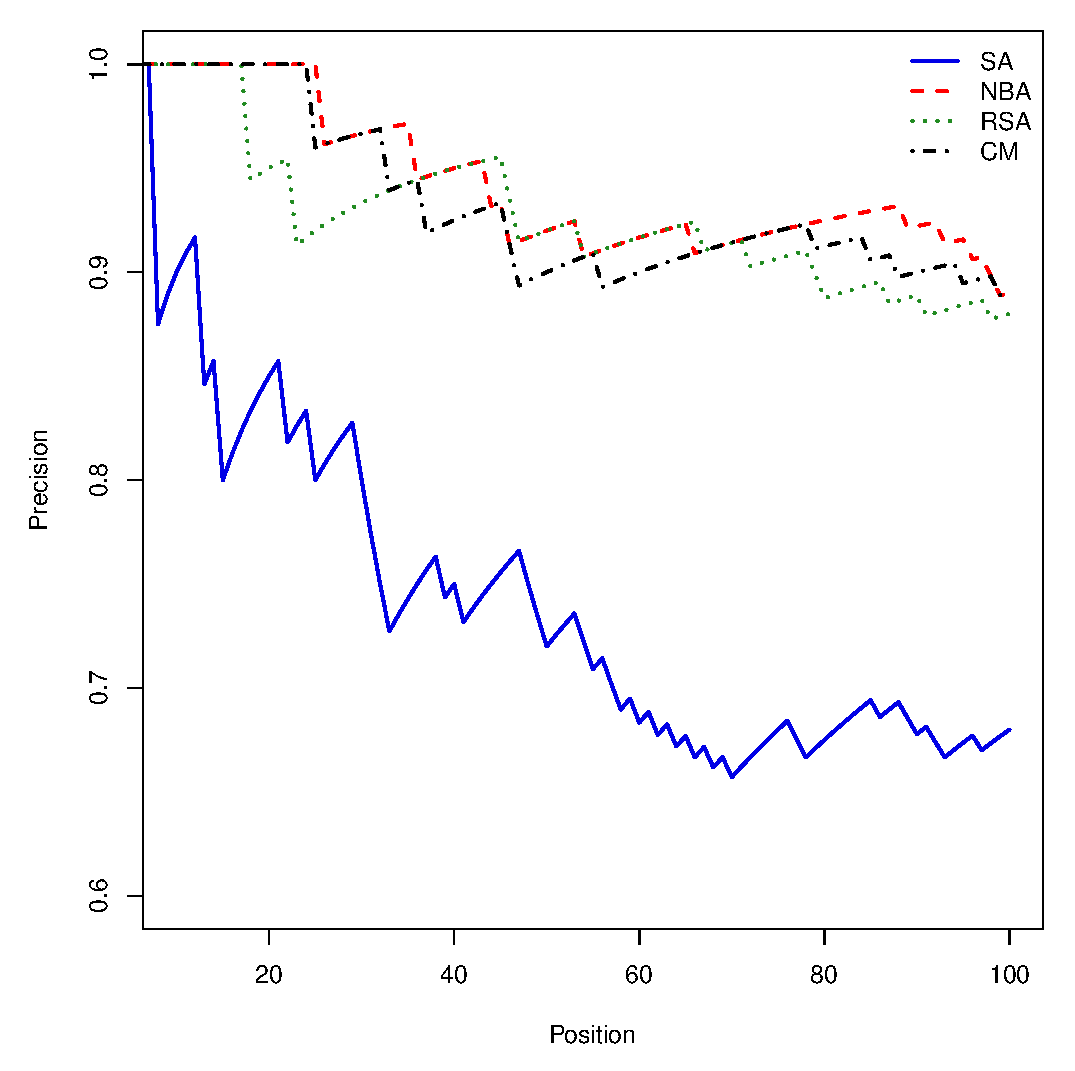
\includegraphics[width=0.45\textwidth]{experiment/e1.ucla.pool.eps}
\caption{Precision@K for UCLA category on human label data.}
\label{fig:e2}
\end{figure}

Moreover, we show some important features generated by NBA in table \ref{tab:keyword}. We ranked the words according to their weight $\log p(c|w)$ and pick up the top $10$ words for different categories. From the table, we could learn some different attributes related to particular category of users. For example, UCLA students like ``dailybruin'' news, call themselves as ``bruins'' and lived near ``westwood''; USC students like tweets from ``usc annenberge'' and the idol statue in their university is ``Trojan''; MIT students live in ``Cambridge'' and there is famous ``media lab'' in their computer science department; Stanford students are glad to talking about their athletic team using nick name ``cardinal''.

\begin{table*}[htb!]
\centering
\begin{tabular}{|l|l|}
\hline
UCLA & dailybruin, bruin, bruins, westwod, neuheisel, alumna, wooden, undergraduate, midterm, royce \\
\hline
USC & ascj, uscedu, annenberg, uscpsycho, uscannenberg, ausc, beattheirish, trojan, trojans, atrojan \\
\hline
MIT & sloan, medialab, cambridge, joi, kayak, bostonupdate, alums, mechanical, techreview, edu \\
\hline
Stanford & stanfordfball, gostanford, astanford, gsb, cardinal, cantor, tristanwalker, auditorium, alums, freshmen \\
\hline
\end{tabular}
\caption{The keywords in short bio and tweets of users from different universities.}\label{tab:keyword}
\end{table*}

\subsection{Ranking with Loss of Information}
In this part of the experiments, we evaluate our different models with the loss of information. The loss of information means that during the training process, we erase some users profile in label data and treat these users as normal users without our target profile keywords. We test our program and plot the results for different amount of training data in Figure \ref{fig:e3}.

\begin{figure}[h]
\centering
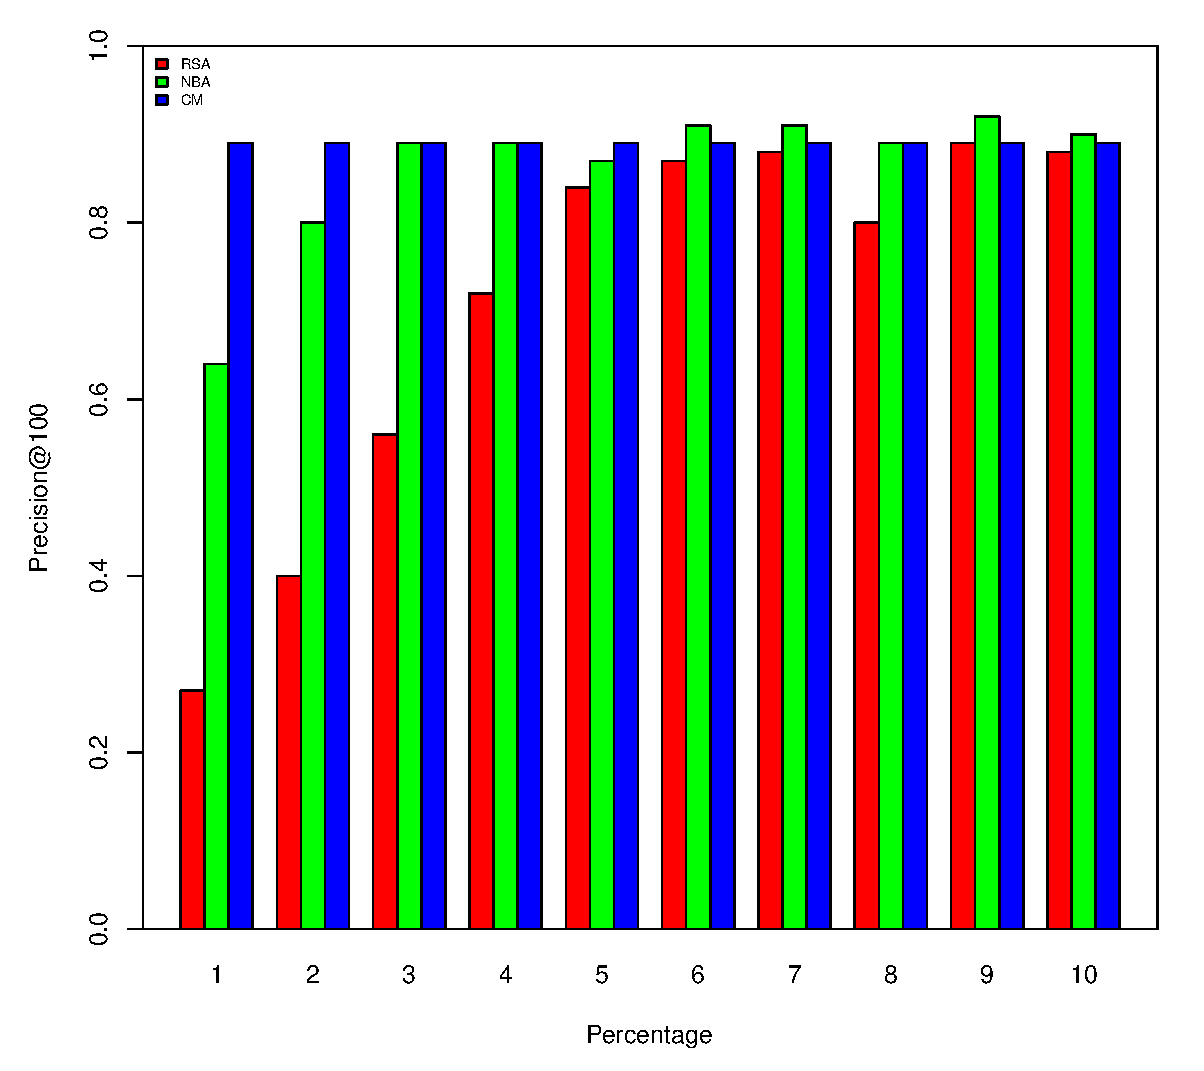
\includegraphics[width=0.45\textwidth]{experiment/e2.ucla.eps}
\caption{Precision@100 for UCLA category with information lost.}
\label{fig:e3}
\end{figure}

The results show that with the loss of information, the performance of RSA falls down dramatically. It also suggests that with few positive training examples, training users in UCLA becomes less connected. The poor graph structure influence the performance of RSA a lot.
Noticed that NBA still have a very good result with $30\%$ positive training examples. Within those percentage of training users, we could already detect the topic among the tweets published by users with UCLA category.

As our expectation, although the ranking of users have little change in CM results, the precision@100 didn't change. When we look inside the ranking result, the top results returned by RSA and NBA are very accurate. So the amount of positive training examples does not affect the ranking result very much.

In our original dataset, the training users are likely to connected with each other since they are in same university. However, for other categories such as father, gamer or phd, users belong to such categories maybe not likely to connected with others in same category. When we erase the profile keyword in label data, the connection in label data become smaller and the structure may like other categories. The performance of our algorithms also demonstrate that our algorithms could be applied to different categories.

\ifx \allfiles \undefined
\end{document}
\fi

%I think we need rewrite this part. Thanks.

%Our crawler will begin with Twitter users from four universities including UCLA, USC, Stanford and MIT, and perform a two-step random walk starting from these users to obtain a larger set of different background users. Every user's profile, followers and followings information will be retrieved. The crawler will also retrieve these users' tweets posted after a specific time.
%We will analysis the number of followers, followings, tweets and retweets for each user, and quantify a user's influence on these metrics using a PageRank like mechanism.
%We will analysis the tweet keywords for each user, and provide a metric to evaluate the tweets similarity between two users. We will also compare the interest difference between users in different universities.
%We will quantify two users' closeness using their tweet and reply (regarding retweet as a kind of reply) behavior data. Our model is similar to the model used in predicting a chess game result based on two players' past campaign results \cite{elo1986rating}.
%We will propose an algorithm for extracting a user's hidden profile. Each edge will be weighted by the closeness and tweets similarity of the corresponding two users. The algorithm performs a random walk on the weighted graph to collect all possible hidden profile for a specific user.
